\section{Revisão Informal}

Nesta seção, serão discutidos alguns trabalhos relacionados ao tema de
categorização fake news, de modo a entender quais são abordagens que estão sendo
propostas na literatura, a qualidade dos resultados obtidos por \xexeoswap{estes}{estas abordagens}, \xexeo[como também, os possíveis impactos sociais, políticos e econômicos que podem ser causados pela disseminação desse tipo de conteúdo]{Se propor a entender isso em um artigo científico significa uma investigação profunda}.

\subsection{\textit{A Survey on Natural Language Processing for Fake News Detection}}

Em \cite{oshikawa2020} os autores conduziram uma pesquisa sobre processamento de linguagem natural para detecção de notícias falsas \xexeo[em que eles forneceram uma visão geral dos esforços de pesquisa para detecção de notícias falsas]{Perceba como essa frase é uma repetição do que você acabou de dizer.} e uma comparação sistemática de suas definições de tarefas, conjuntos de dados, construção de modelos, e performances. \xexeorem[Em geral, não vejo ``Em suma'' em artigos, mas, em todo caso, ele só seria usado como uma ligação da sentença com várias coisas que você já escreve, e não para sumarizar o que vai falar.]{Em suma,} suas contribuições gerais foram \xexeo[as seguintes]{pode parar no foram, não precisa do as seguintes}: 

\begin{enumerate}
    \item \xexeoswap{Fornecer uma revisão das}{Revisar as} soluções de processamento de linguagem natural para detecção automática de notícias falsas.
    
    \item Analisar sistematicamente como a detecção de notícias falsas estão alinhadas com as tarefas de \textit{NLP} existentes e \xexeoswap[mantenha os verbos na mesma pessoa tempo]{discutiram}{discutir} as suposições e questões notáveis para diferentes formulações do problema;
    
    \item Categorizar e resumir os \textit{datasets} disponíveis, abordagens de \textit{NLP} e resultados, fornecendo \xexeo[experiências em primeira mão]{Não li, mas como uma revisão oferece uma experiência em primeira mão?} e introduções acessíveis para novos pesquisadores interessado neste problema.
\end{enumerate}

\subsubsection{Problemas Relacionados a detecção de \textit{fake news}}

A respeito de problemas relacionados a detecção automática de \textit{fake news}, os autores destacaram\xexeorem{4 que são eles}:\xexeo{Se colocou o dois pontos, ou segue a linha ou itemiza.} 

\begin{itemize}
\item \textbf{\textit{Fact-Checking}} Em geral, a detecção de \textit{fake news} usualmente foca em eventos novos, enquanto \textit{fact-checking} é mais amplo. 
Vale resaltar que, segundo os autores, muitos pesquisadores não distinguem detecção de \textit{fake news} e \textit{fact-checking}, pois ambos visam avaliar a veracidade de alegações;  

\item \textbf{\textit{Rumor Detection}} Não há uma definição consistente de detecção de rumor. Uma pesquisa recente (\cite{zubiaga2018}) define detecção de boatos\xexeo{Boato ou rumor, o leitor já se confundiu} como separar declarações pessoais em boatos ou não boatos, onde o boato é definido como uma declaração que consiste em informações não verificadas no momento da postagem. \xexeo[Dentro de outras palavras]{Se você queria dizer ``em poucas palavras'', não se usa em artigos}, o boato deve conter informações que possam ser verificados em vez de opiniões ou sentimentos subjetivos; 


\item  \textbf{\textit{Stance Detection}} é definida como a tarefa de aferir de qual lado de um debate um autor está no texto. Isto difere de detecção de \textit{fake news} no sentido que não se trata sobre a veracidade, mas da consistência. 
 \textit{Stance Detection} pode ser uma subtarefa de detecção de \textit{fake news} pois ela pode ser aplicada para buscar documentos para evidência; 


\textbf{\textit{Sentiment Analysis}} A análise de sentimentos é a tarefa de extrair emoções, como impressão favorável ou desfavorável dos clientes de um restaurante. Diferente da detecção de boatos e de notícias falsas, a análise de sentimento não é fazer uma verificação objetiva de alegações, mas \xexeorem{para} analisar as emoções pessoais. 

\end{itemize}

\subsubsection{Formulações das tarefas}

Existem diferentes tipos de estratégias de rotular ou avaliar a detecção de \textit{fake news}. 
Na maior parte dos estudos, a Detecção de \textit{Fake News} é formulada como um problema de classificacão ou de regressão\xexeo{Acho impossível ser uma tarefa de regressão, me explica isso, lembrando que se foi usada regressão Logística não é regressão}, entretanto a abordagem do problema de classificação é mais frequentemente utilizada. 

\textbf{Classificação} A maneira mais comum de formular o problema de detecção de \textit{fake news} é como um problema de classificação binária. Todavia, categorizar todas as notícias dentro de apenas duas classes (\textit{fake} ou \textit{real}) é difícil devido a existência de casos em que uma notícia pode ser parcialmente verdadeira e, simultaneamente, parcialmente falsa. Para endereçar este problema, acrescentar classes adicionais é uma prática comum. Principalmente, uma categoria para \textit{fake news} que não são  completamente verdadeiras ou completamente falsas, ou então \xexeorem{são inseridos} categorias para representar diferentes graus de veracidade que as notícias podem conter. \\


\textbf{Regressão} A Detecção de \textit{fake news} também pode ser formulada como uma tarefa de regressão\xexeo{Dei uma olhada no artigo e não acho que seja uma tarefa de regressão}, onde a saída será uma pontuação numérica que representa a veracidade da informação. Esta abordagem é utlizada por \cite{nakashole2014}. Geralmente, a avaliação é feita através do calculo da diferença entre as pontuações preditas e o piso da pontuação de veracidade ou então usando, \textit{Correlações de Pearson/Spearman}. No entanto, uma vez que os conjuntos de dados disponíveis possuem pontuações discretizadas de veracidade, o desafio aqui é como converter os rótulos discretos para pontuações numéricas continuas. 


\subsection{Social Media and Fake News in the 2016 Election}

\subsubsection{Definição}

\cite{allcot2017} Definiram  \textit{fake news} como artigos que são intencionalmente e verificavelmente falsos, e podem enganar os leitores. 
Esta definição inclui \xexeosug{tanto} artigos fabricados intencionalmente por websites como por exemplo \textit{denverguardian.com}, \xexeo[como também]{exige alguma como ``tanto'' na sentença anterior} artigos oriundos de \textit{websites} satíricos que podem ser mal interpretados como fatuais, especialmente quando vistos isolados nas redes sociais, como \xexeorem{no} \textit{Twitter} ou \textit{Facebook}. Esta definição exclui diversos ``parentes próximos'' de \textit{fake news} como por exemplo:

\begin{enumerate}
    \item Erros não intencionais de relatórios;
    \item Rumores que não se originam de uma determinada notícia;
    \item Teorias da conspiração (estas são, por definição, difíceis de verificar como verdadeiras ou falsas, e são tipicamente originadas por pessoas que acreditam que elas sejam verdadeiras);
    \item Sátira, que dificilmente será interpretado erroneamente como fatual;
    \item Declarações falsas de políticos;
    \item Relatórios que são enviesados ou enganosos, mas não totalmente falsos.
\end{enumerate}


\subsubsection{Quem produz \textit{fake news}?}

Parecem existir duas motivações principais para disseminação de \textit{fake news}. 
A primeira é pecuniária: artigos de notícias que se tornam virais nas mídias sociais podem atrair anúncios significativos aumentar a receita quando os usuários clicam no site original. 
Esta parece ter sido a principal motivação para a maioria dos produtores cujas identidades foram reveladas. 
A segunda motivação é ideológica. 
Alguns provedores de notícias falsas procuram promover os candidatos que preferem.


\subsubsection{Um Modelo de \textit{Fake News}}


De forma mais ampla, como \textit{fake news} diferem de dados tendenciosos ou enviesados? É uma forma inócua de entretenimento, como filmes de ficção ou romances? Ou têm maiores custos sociais? 

Para responder a estas pergntas, \cite{allcot2017} esboçaram um modelo baseado de demanda por notícias baseado em um modelo desenvolvido formalmente em \cite{gentzkow2016}\xexeo{Interessante, mas primeiro está confuso e segundo não avança na direção da sua proposta, logo, se não vai usar, porque falar?}. 

Existem dois possíveis estados não observados do mundo, que podem representar se um candidato de esquerda ou de direita terá melhor desempenho no cargo. 
Empresas de mídia recebem sinais que são informativos sobre o estado verdadeiro e podem diferir na
precisão desses sinais. 
Também podemos imaginar que as empresas podem fazer investimentos dispendiosos para aumentar a precisão desses sinais. 
Cada empresa tem uma estratégia de relatórios que mapeia desde os sinais que recebe até as notícias que publica. 
Empresas podem decidir relatar os sinais com veracidade ou, alternativamente, adicionar viés aos relatórios. 

No modelo proposto, os consumidores devem escolher uma ação, que poderia
representar defender ou votar em um candidato, e recebem benefícios privados se
eles escolhem o candidato que prefeririam se estivessem plenamente informados. 
Segundo\xexeo{Segundo quem? O que?},
consumidores podem derivar utilidade psicológica de ver relatórios que são consistentes com suas ideologias. 
Os consumidores escolhem as empresas das quais consumirão notícias
para maximizar sua própria utilidade esperada. 
Eles então usam o conteúdo das notícias que consumiram para formar um conceito sobre o estado do mundo. 

Nesse modelo, dois incentivos distintos podem levar as empresas a distorcer seus relatórios na direção das ideologias dos consumidores. 
Primeiro, quando o feedback sobre o verdadeiro estado é limitado,
consumidores racionais julgarão uma empresa de melhor qualidade quando seus relatórios estiverem mais próximos
de suas ideologias. 
Em segundo lugar, os consumidores podem preferir relatórios que confirmem suas ideologias. 

Produtores de notícias falsas são empresas com duas características distintas. Primeiro, eles não fazem
investimento em relatórios precisos, de modo que seus sinais subjacentes não sejam correlacionados com
o verdadeiro estado. 
Em segundo lugar, eles não tentam construir uma reputação de qualidade para longo prazo, mas sim maximizar os lucros de curto prazo de atrair cliques em um determinado período. 

Adicionar produtores de notícias falsas a um mercado tem vários custos sociais potenciais. 
Primeiro,
consumidores que confundem uma saída falsa com uma legítima têm crenças menos precisas
e são piores por esse motivo. Em segundo lugar, essas crenças menos precisas podem reduzir
externalidades sociais positivas, minando a capacidade do processo democrático de
selecionar candidatos de alta qualidade. Terceiro, os consumidores também podem se tornar mais céticos
de produtores legítimos de notícias, na medida em que se tornam difíceis de distinguir
de produtores de notícias falsas. Quarto, esses efeitos podem ser reforçados em equilíbrio por
respostas do lado da oferta: uma demanda reduzida por relatórios de alta precisão e baixo viés
reduziria os incentivos para investir em relatórios precisos e sinais de relatórios com veracidade.
Esses efeitos negativos sobrepõem-se diante de qualquer ganho de bem-estar que surja dos consumidores
que gostam de ler notícias falsas consistentes com seus antecedentes.


\subsection{\textit{Fake News detection Using Machine Learning}}

Em \cite{baarir2020} os autores apresentam um método para detecção de \textit{fake news} que utiliza: 
\begin{enumerate}
    \item \textbf{Pré-processamento de texto} que consiste do uso de \textit{stemmers}, remoção de \textit{stop words} e caracteres especiais;
    \item \textbf{\textit{Encoding} do texto} utilizando modelos de \textit{bag of words}, \textbf{N-gram} e \textit{TF-IDF}
    \item \textbf{Extração de características} que permite uma identificação precisa de informações falsas. Foram utilizados como \textit{features} a fonte da notícia, o autor, a data e o sentimento do texto.
    \item \textbf{\textit{Support Vector Machine}} Um algoritmo de aprendizado de máquina supervisionado vastamente utilizado em problemas de classificação.
\end{enumerate}


\subsubsection{Sistema proposto}

O sistema proposto\xexeo{Nunca fale de um trabalho de outro como sistema proposto, pois quando um leitor vê essas palavras imediatamente começa a ler como se fosse sua proposta} usa como entrada uma base de dados de comentários e metadados, tais como, data, fonte e autor. 
Essa informação era\xexeo{mudou o tempo do verbo. Era ``usa'', virou ``era''} então transformada em \textit{features} que podiam ser usadas na etapa de aprendizagem. 

A base de dados processada era dividida em duas partes: a primeira, que é utilizada para treinamento, e a segunda, que é utilizada para teste\xexeo{Isso é uma explicação ingênua de um tratamento padrão, base de treinamento e teste.}. 
O \xexeo[modulo de treinamento utiliza os dados de treinamento]{Não é óbvio, reforçar esse conceito faz o leitor acreditar que você é um usuário ingênuo} e o algoritmo \textit{SVM} para construir um modelo de decisão \xexeo[que pode ser aplicado a base de dados de teste]{Ainda óbvio}. Se o modelo for aceito, isto é, for capaz de alcançar um nível de acurácia aceitável, ele pode ser mantido e utilizado quando o treinamento terminar. Caso contrário, os parâmetros do algoritmo de aprendizado são \xexeo[tunados]{Essa palavra está proibida em artigos!} de modo a aprimorar a acurácia do modelo. O modelo proposto pode ser visto na Figura \ref{fig:mesh1}.\xexeo{Tudo isso é tão padrão que não merece ser descrito. Algo como ``Dividindo a base entre um conjunto de aprendizado e um conjunto de testes, o autor obtém um modelo com a aplicação do algoritmo SVM na primeira base, que deve atingir uma acurácia aceitável quando usado na segunda base''}

\begin{figure}[h]
    \centering
    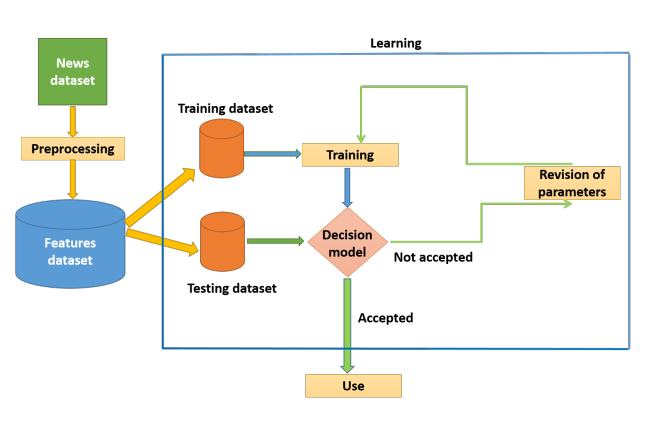
\includegraphics[width=0.5\textwidth]{Imagens/revisao informal/modelo1.png}
    \caption{Modelo de aprendizado}
    \label{fig:mesh1}
\end{figure}

\subsubsection{Pré-processamento}

Na base de dados utilizada, as características das noticias são classificadas em três categorias: dados textuais, dados categóricos e dados numéricos. \\

\textbf{Dados Textuais}: Estes são os dados que representam o texto escrito pelo autor. O pré-processamento desses dados consiste das seguintes operações: \\

\begin{enumerate}
    \item \textbf{Limpeza}: Elimina \textit{stop words} e caracteres especiais;
    \item \textbf{\textit{Steming}}: Transforma as palavras úteis em radicais\xexeo{Você está dizendo que o stemmer faz stemming, tem que explicar melhor se for explicar};
    \item \textbf{\textit{Encoding}}: transforma todas as palavras do texto em um vetor numérico. Esta etapa necessita de dois passos: A combinação de duas técnicas, especificamente, \textit{bag-of-words} \cite{gerard1983} e \textit{N-grams} \cite{chris1985}, então a aplicação do método \textit{TF-IDF} \cite{juan2003} no resultado.\xexeo{ok, não estou lendo o artigo, mas não é transforma, é associa} 
\end{enumerate} 


\textbf{Dados Categóricos}: 


Dados categóricos. Representam a fonte das notícias tais como canal de TV, jornal ou revista, e seu autor. O pré-tratamento desses dados é realizado através de dois passos:
\begin{enumerate}
    \item \textbf{Limpeza}: eliminando caracteres especiais e transformando os caracteres para \textit{lowercase}.
    \item \textbf{Codificação}:  para fontes foram utilizados uma codificação de \textit{labels}. Por autores, foi criada uma codificação para converter os nomes do autor em números digitais, de modo que autores da mesma fonte estão próximos uns dos outros comparação com autores de outras fontes. 
\end{enumerate}


\textbf{Dados Numéricos}: Representam a data da notícia e o sentimento dado pelo texto. A data foi utilizada como 3 valores numéricos distintos, o dia, o mês e o ano da postagem da notícia. 

\textbf{Sentimento} Para o sentimento dado pelo texto, foi calculado a soma dos graus de sentimento das palavras. De acordo com experts, cada palavra possui um grau de sentimento que permite com que ela seja classificada em três classes: \textit{(i)} Se a soma for menor que zero, o sentimento é negativo; \textit{(ii)} Se a soma for maior que zero, o sentimento é positivo; \textit{(iii)} se a somar for 0, o sentimento é neutro.


\subsubsection{\textit{Dataset}}

O \textit{Dataset} utilizado foi uma combinação de dois outros existentes  "Getting Real about
Fake News" \cite{fakenews2016} e "All the news" \cite{allthenews2017}. 
Estes \textit{datasets} foram obtidos do website \textit{Kaggle}. 
Após pré-processar os dois conjuntos de dados e testar os recursos um a um até atingir a melhor taxa de precisão. 

Foi obtido um conjunto de dados que contém as seguintes características:

\begin{itemize}
    \item 5 palavras obtidas pelo método \textit{bag of words},
    \item 3 palavras compostas obtidas pelo método \textit{N-gram},
    \item Data: dia, mês e ano,
    \item Sentimento,
    \item Fonte,
    \item Autor,
    \item Classe: falsa ou real. \\
\end{itemize}

\subsubsection{Resultados}
Este artigo apresentou um método de detecção de notícias falsas usando o algoritmo SVM, tentando determinar os melhores recursos e técnicas para detectar notícias falsas.\xexeo{Não é uma conclusão do seu artigo, você já explicou isso} Por meio da pesquisa realizada durante este estudo, os autores obtiveram os seguintes resultados:

\begin{itemize}
    \item A influencia da \textit{feature} "sentimento"\xexeo{veja no texto anterior como fazer aspas no \LaTeX} na acurácia foi quase insignificante, o que parece ser bem lógico, pois uma notícia ter um sentimento positivo ou negativo não está relacionado com a veracidade de sua informação.
    \item Os melhores recursos para detectar notícias falsas estão em ordem: texto, autor, fonte, data e sentimento.
    \item o método N-gram dá um resultado melhor do que o \textit{bag of words} com conjuntos de dados volumosos e com textos grandes\xexeo{Qual o n? O N word também gera um bag normalmente};
    \item O \textit{SVM} parece ser o melhor algoritmo para detectar notícias falsas, porque deu uma melhor taxa de reconhecimento, e permitiu a dar para cada informação um grau de confiança para a sua classificação\xexeo{Você não citou outros}.
    \item os parâmetros que mais influenciam o SVM são respectivamente: Custo C, gama $\gamma$ e épsilon $\epsilon$. \xexeo{Isso tá ruim, além disso tem o kernel que deve ser super importante, que kernel foi usado}
    \end{itemize}
